\begin{name}
	{\tenchude}{\tendethi}{LỚP TOÁN THẦY PHÁT}{\thoigian}
\end{name}
\setcounter{ex}{0}\setcounter{bt}{0}
\Opensolutionfile{ans}[ans/ans-2-TT-17-SGD-HaNoi-23]
\begin{ex}%[Dự án 12EX6-2023]%[Đề thi thử SGD Hà Nội 2023, Nguyễn Anh Quốc]%[2H1Y1-1]
	\immini{Số cạnh của một hình đa diện như hình vẽ dưới đây là	
		\choice
		{\True $12$}
		{$10$}
		{$16$}
		{$8$}}
	{\begin{tikzpicture}[scale=0.5,>=stealth, font=\footnotesize, line join=round, line cap=round]
		\tkzDefPoints{0/0/A,-1.9/-1.6/B,1.6/-1.6/C}
		\coordinate (D) at ($(A)+(C)-(B)$);
		\coordinate (O) at ($(A)!1/2!(C)$);
		\coordinate (S) at ($(O)+(0,3.5)$);
		\coordinate (N) at ($(O)!-1!(S)$);
		
		\tkzDrawPolygon(S,B,C,D)
		\tkzDrawSegments(S,C B,N D,N C,N)
		\tkzDrawSegments[dashed](A,S A,B A,D A,N)
		\end{tikzpicture}}
	\loigiai{
		Số cạnh của hình đa diện là $12$.	
	}
\end{ex}

\begin{ex}%[Dự án 12EX6-2023]%[Đề thi thử SGD Hà Nội 2023, Nguyễn Anh Quốc]%[2H3Y2-2]
	Trong KG $Oxyz$, một véc-tơ pháp tuyến của mặt phẳng $(\alpha)\colon x+2y-4z+2=0$ có tọa độ là	
	\choice
	{$(1;-2;4)$}
	{$(1;2;4)$}
	{$(-1;2;4)$}
	{\True $(1;2;-4)$}
	\loigiai{
		Véc-tơ pháp tuyến của mặt phẳng $(\alpha)$ là $\overrightarrow{n}=(1;2;-4)$.	
	}
\end{ex}

\begin{ex}%[Dự án 12EX6-2023]%[Đề thi thử SGD Hà Nội 2023, Nguyễn Anh Quốc]%[2D1Y3-1]
	\immini{Cho hàm số $y=f(x)$ liên tục trên đoạn $[-1;3]$ và có đồ thj như hình vẽ. Giá trị lớn nhất của hàm số đã cho trên đoạn $[-1;3]$ bằng	
		\choice
		{$3$}
		{$-1$}
		{\True $4$}
		{$2$}}
	{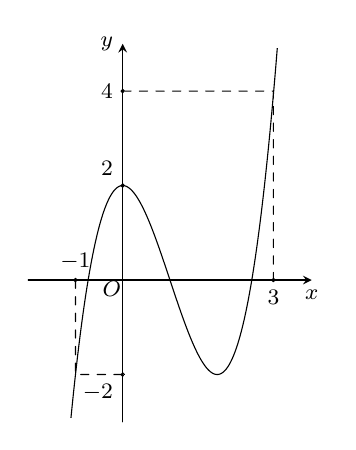
\begin{tikzpicture}[scale=0.6, font=\footnotesize, line join=round, line cap=round, >=stealth]
		\def\a{1} \def\b{-3} \def\c{0} \def\d{2}
		\def\xmin{-2} \def\xmax{4}
		\def\ymin{-3} \def\ymax{5}
		%	\draw[color=gray!50,dashed] (\xmin,\ymin) grid (\xmax,\ymax);
		\draw[->] (\xmin,0)--(\xmax,0) node [below]{$x$};
		\draw[->] (0,\ymin)--(0,\ymax) node [left]{$y$};
		\node at (0,0) [below left=-3pt]{$O$};
		\clip (\xmin+0.1,\ymin+0.1) rectangle (\xmax-0.2,\ymax-0.1);
		\draw[samples=200,domain=\xmin+0.1:\xmax-0.2] plot(\x,{\a*(\x)^3+\b*(\x)^2+\c*(\x)+\d});
		\draw[dashed](-1,0)node[above]{$-1$}circle(1pt)--(-1,-2)--(0,-2)node[below left]{$-2$}circle(1pt) (0,2)node[above left]{$2$}circle(1pt) (0,4)node[left]{$4$}circle(1pt)--(3.19,4)--(3.19,0)node[below]{$3$}circle(1pt);
		
		\end{tikzpicture}
	}
	\loigiai{
		Dựa vào đồ thị hàm số ta thấy giá trị lớn nhất của hàm số trên $[-1;3]$ là $4$.	
	}
\end{ex}

\begin{ex}%[Dự án 12EX6-2023]%[Đề thi thử SGD Hà Nội 2023, Nguyễn Anh Quốc]%[2H2Y1-2]
	Diện tích xung quanh của hình nón có đường sinh $\ell$ và bán kính đáy $r$ bằng	
	\choice
	{\True $\pi r\ell$}
	{$\pi r(\ell+r)$}
	{$\pi^2r\ell$}
	{$2\pi r\ell$}
	\loigiai{
		Diện tích xung quanh của hình nón là $S=\pi r\ell$.	
	}
\end{ex}

\begin{ex}%[Dự án 12EX6-2023]%[Đề thi thử SGD Hà Nội 2023, Nguyễn Anh Quốc]%[2H3Y1-1]
	Trong KG $Oxyz$, cho $\overrightarrow{a}=-2\cdot \overrightarrow{i}+2\cdot \overrightarrow{j}-3\cdot\overrightarrow{k}$. Tọa độ của véc-tơ $\overrightarrow{a}$ là	
	\choice
	{$(2;-2;-3)$}
	{\True $(-2;2;-3)$}
	{$(2;-2;3)$}
	{$(2;2;-3)$}
	\loigiai{
		Ta có $\overrightarrow{a}=-2\cdot \overrightarrow{i}+2\cdot \overrightarrow{j}-3\cdot\overrightarrow{k}\Leftrightarrow \overrightarrow{a}=(-2;2;-3).$	
	}
\end{ex}

\begin{ex}%[Dự án 12EX6-2023]%[Đề thi thử SGD Hà Nội 2023, Nguyễn Anh Quốc]%[2D1Y2-2]
	Cho hàm số $y=f(x)$ có bảng biến thiên như hình bên dưới
	\begin{center}
		
\begin{tikzpicture}
		\tkzTabInit[nocadre=false,lgt=1.2,espcl=2.5,deltacl=0.6]
		{$x$/0.6, $f'(x)$/0.6, $f(x)$/2}
		{$-\infty$,$-2$,$3$,$+\infty$}
		\tkzTabLine{,-,$0$,+,$0$,-,}
		\tkzTabVar{+/$+\infty$,-/$-3$,+/$2$,-/$-\infty$}
		\end{tikzpicture}
	\end{center}
	Giá trị cực đại của hàm số đã cho bằng
	\choice
	{$-3$}
	{$-2$}
	{\True $2$}
	{$3$}
	\loigiai{
		Dựa vào bảng biến thiên ta thấy hàm số đã cho có giá trị cực đại bằng $2$.	
	}
\end{ex}

\begin{ex}%[Dự án 12EX6-2023]%[Đề thi thử SGD Hà Nội 2023, Nguyễn Anh Quốc]%[2D2Y4-3]
	Trong các hàm số dưới đây, hàm số nào nghịch biến trên tập $\mathbb{R}?$	
	\choice
	{$y=\log_3x$}
	{\True $y=\left(\dfrac{2}{\mathrm{e}}\right)^x$}
	{$y=\left(\dfrac{\pi}{3}\right)^x$}
	{$\log_{\frac{1}{2}}x$}
	\loigiai{
		Hàm số $y=\left(\dfrac{2}{\mathrm{e}}\right)^x$ có tập xác định là $\mathscr{D}=\mathbb{R}$ và $\dfrac{2}{\mathrm{e}}<1$ nên hàm số đã cho nghịch biến trên $\mathbb{R}$.
	}
\end{ex}

\begin{ex}%[Dự án 12EX6-2023]%[Đề thi thử SGD Hà Nội 2023, Nguyễn Anh Quốc]%[2H2Y1-1]
	Thể tích của khối trụ có bán kính đáy $r$ và chiều cao $h$ bằng	
	\choice
	{\True $\pi r^2 h$}
	{$2\pi rh$}
	{$\pi rh$}
	{ $\dfrac{1}{3}\pi r^2 h$}
	\loigiai{
		Thể tích của khối trụ là $V=\pi r^2 h$.	
	}
\end{ex}

\begin{ex}%[Dự án 12EX6-2023]%[Đề thi thử SGD Hà Nội 2023, Nguyễn Anh Quốc]%[1D2Y2-1]
	Số cách chọn $5$ học sinh bất kì từ $12$ học sinh bằng	
	\choice
	{$5^{12}$}
	{\True $\mathrm{C}^5_{12}$}
	{$\mathrm{A}^5_{12}$}
	{$12^5$}
	\loigiai{
		Chọn $5$ học sinh từ $12$ học sinh là một tổ hợp chập $5$ của $12$ phần tử nên số cách chọn là $\mathrm{C}^5_{12}$.	
	}
\end{ex}

\begin{ex}%[Dự án 12EX6-2023]%[Đề thi thử SGD Hà Nội 2023, Nguyễn Anh Quốc]%[2H3Y1-3]
	Trong KG $Oxyz$, mặt cầu tâm $I(1;4;2)$ và bán kính $R=2$ có phương trình là 	
	\choice
	{\True $(x-1)^2+(y-4)^2+(z-2)^2=4$}
	{$(x+1)^2+(y+4)^2+(z-2)^2=2$}
	{$(x+1)^2+(y+4)^2+(z-2)^2=4$}
	{$(x-1)^2+(y-4)^2+(z-2)^2=2$}
	\loigiai{
		Phương trình mặt cầu tâm $I(1;4;2)$ và bán kính $R=2$ là $$(x-1)^2+(y-4)^2+(z-2)^2=4.$$	
	}
\end{ex}

\begin{ex}%[Dự án 12EX6-2023]%[Đề thi thử SGD Hà Nội 2023, Nguyễn Anh Quốc]%[2D1Y4-1]
	Đường tiệm cận đứng của đồ thị hàm số $y=\dfrac{x-1}{x+1}$ là
	\choice
	{$y=1$}
	{$x=1$}
	{\True $x=-1$}
	{$y=-1$}
	\loigiai{
		Ta có $\displaystyle\lim_{x\to -1^+}\dfrac{x-1}{x+1}=-\infty$ nên $x=-1$ là tiệm cận đứng của đồ thị hàm số.	
	}
\end{ex}

\begin{ex}%[Dự án 12EX6-2023]%[Đề thi thử SGD Hà Nội 2023, Nguyễn Anh Quốc]%[2D1Y5-1]
	\immini{Hàm số nào dưới đây có đồ thị như hình vẽ bên?	
		\choice
		{$y=-2x^2-1$}
		{$y=x^4-2x^2$}
		{$y=x^3-2x^2+2$}
		{\True $y=\dfrac{2x-3}{x-1}$}}
	{
		\begin{tikzpicture}[scale=1, font=\footnotesize, line join=round, line cap=round, >=stealth]
		\def\a{2} \def\b{-3} \def\c{1} \def\d{-1}
		\def\xmin{-3} \def\xmax{4}
		\def\ymin{-2} \def\ymax{5}
		%\draw[color=gray!50,dashed] (\xmin,\ymin) grid (\xmax,\ymax);
		\draw[->] (\xmin,0)--(\xmax,0) node [below]{$x$};
		\draw[->] (0,\ymin)--(0,\ymax) node [left]{$y$};
		\node at (0,0) [below left=-3pt]{$O$};
		\clip (\xmin+0.1,\ymin+0.1) rectangle (\xmax-0.1,\ymax-0.1);
		\draw[samples=200,domain=\xmin:(-\d/\c-0.1)] plot(\x,{(\a*(\x)+\b)/(\c*(\x)+\d)});
		\draw[samples=200,domain=(-\d/\c+0.1:\xmax)] plot(\x,{(\a*(\x)+\b)/(\c*(\x)+\d)});
		\draw[dashed] (-\d/\c,\ymin)--(-\d/\c,\ymax);
		\draw[dashed] (\xmin,\a/\c)--(\xmax,\a/\c);
		\end{tikzpicture}
		
	}
	\loigiai{
		Đồ thị đã cho là đồ thị hàm số nhất biến nên ta chọn $y=\dfrac{2x-3}{x-1}$.
	}
\end{ex}

\begin{ex}%[Dự án 12EX6-2023]%[Đề thi thử SGD Hà Nội 2023, Nguyễn Anh Quốc]%[2D3Y3-3]
	Cho hình phẳng $(H)$ giới hạn bởi đồ thị hàm số $y=f(x)$, trục $Ox$ và các đường thẳng $x=a$, $x=b$ $(a<b)$. Gọi $V$ là thể tích khối tròn xoay thu được khi cho $(H)$ quay quanh trục $Ox$. Khẳng định nào sau đây đúng?	
	\choice
	{$V=\displaystyle\int^b_a\left|f(x)\right|\mathrm{\,d}x$}
	{$V=\pi \displaystyle\int^b_a\left|f(x)\right|\mathrm{\,d}x$}
	{\True $V=\pi\displaystyle\int^b_af^2(x)\mathrm{\,d}x$}
	{$V=\displaystyle\int^b_af^2(x)\mathrm{\,d}x$}
	\loigiai{
		Thể tích của khối tròn xoay được tính theo công thức $V=\pi\displaystyle\int^b_af^2(x)\mathrm{\,d}x$.	
	}
\end{ex}

\begin{ex}%[Dự án 12EX6-2023]%[Đề thi thử SGD Hà Nội 2023, Nguyễn Anh Quốc]%[2D2Y1-2]
	Với mọi số thực $\alpha$, $\beta$ và số dương $a$ khác $1$, khẳng định nào sau đây \textbf{sai}?	
	\choice
	{$a^{\alpha}a^{\beta}=a^{\alpha+\beta}$}
	{\True $a^{\alpha}a^{\beta}=a^{\alpha\beta}$}
	{$\left(a^{\alpha}\right)^{\beta}=a^{\alpha\beta}$}
	{$\dfrac{a^{\alpha}}{a^{\beta}}=a^{\alpha-\beta}$}
	\loigiai{
		Khẳng định sai là $a^{\alpha}a^{\beta}=a^{\alpha\beta}$.	
	}
\end{ex}

\begin{ex}%[Dự án 12EX6-2023]%[Đề thi thử SGD Hà Nội 2023, Nguyễn Anh Quốc]%[2D1Y1-2]
	Cho hàm số $y=f(x)$ có bảng xét dấu $f'(x)$ như hình bên dưới
	\begin{center}
		
\begin{tikzpicture}
		\tkzTabInit[nocadre=false,lgt=1.2,espcl=2.5,deltacl=0.6]
		{$x$/0.6, $f'(x)$/0.6}
		{$-\infty$,$-1$,$1$,$+\infty$}
		\tkzTabLine{,-,$0$,+,$0$,-,}
		\end{tikzpicture}
	\end{center}
	Hàm số đã cho đồng biến trên khoảng nào dưới đây?
	\choice
	{$(0;2)$}
	{\True$(-1;1)$}
	{$(1;+\infty)$}
	{$(-\infty;-1)$}
	\loigiai{
		Dựa vào bảng xét dấu ta thấy hàm số đồng biến trong $(-1;1)$.	
	}
\end{ex}

\begin{ex}%[Dự án 12EX6-2023]%[Đề thi thử SGD Hà Nội 2023, Nguyễn Anh Quốc]%[2D3Y1-1]
	Khẳng định nào sau đây \textbf{sai}?	
	\choice
	{$\displaystyle\int \mathrm{e}^x\mathrm{\,d}x=\mathrm{e}^x+C$}
	{$\displaystyle\int x\mathrm{\,d}x=\dfrac{x^2}{2}+C$}
	{\True $\displaystyle\int \dfrac{1}{x}\mathrm{\,d}x=\ln x+C$}
	{$\displaystyle\int \mathrm{\,d}x=x+C$}
	\loigiai{
		Mệnh đề sai là 	$\displaystyle\int \dfrac{1}{x}\mathrm{\,d}x=\ln x+C$.
	}
\end{ex}

\begin{ex}%[Dự án 12EX6-2023]%[Đề thi thử SGD Hà Nội 2023, Nguyễn Anh Quốc]%[2D3Y2-1]
	Nếu $\displaystyle \int^6_2f(x)\mathrm{\,d}x=7$ và $\displaystyle\int^6_2g(x)\mathrm{\,d}x=-2$ thì $\displaystyle\int^6_2\left[f(x)+g(x)\right]\mathrm{\,d}x$ bằng
	\choice
	{\True $5$}
	{$-5$}
	{$-9$}
	{$9$}
	\loigiai{
		Ta có $\displaystyle\int^6_2\left[f(x)+g(x)\right]\mathrm{\,d}x=\displaystyle \int^6_2f(x)\mathrm{\,d}x+\displaystyle \int^6_2g(x)\mathrm{\,d}x=7-2=5.$	
	}
\end{ex}

\begin{ex}%[Dự án 12EX6-2023]%[Đề thi thử SGD Hà Nội 2023, Nguyễn Anh Quốc]%[2D3Y1-1]
	Với hàm số $f(x)$ tùy ý, hàm số $F(x)$ là một nguyên hàm của hàm số $f(x)$. Khẳng định nào sau đây đúng?
	\choice
	{$f'(x)=F(x)$}
	{$F(x)=f(x)$}
	{\True $F'(x)=f(x)$}
	{$F'(x)=f'(x)$}
	\loigiai{
		Ta có $F'(x)=f(x)$.	
	}
\end{ex}

\begin{ex}%[Dự án 12EX6-2023]%[Đề thi thử SGD Hà Nội 2023, Nguyễn Anh Quốc]%[2D3Y2-1]
	Cho các hàm số $f(x)$ và $F(x)$ liên tục trên $\mathbb{R}$ thỏa mãn $F'(x)=f(x)$, $\forall x\in \mathbb{R}$ và $F(0)=2$, $F(1)=6$. Khi đó $\displaystyle\int ^1_0f(x)\mathrm{\,d}x$ bằng	
	\choice
	{$8$}
	{$-8$}
	{$-4$}
	{\True $4$}
	\loigiai{
		Ta có $\displaystyle\int ^1_0f(x)\mathrm{\,d}x=F(x)\bigg|^1_0=F(1)-F(0)=6-2=4.$	
	}
\end{ex}

\begin{ex}%[Dự án 12EX6-2023]%[Đề thi thử SGD Hà Nội 2023, Nguyễn Anh Quốc]%[2D1B5-4]
	\immini{Cho hàm số bậc bốn $y=f(x)$ có đồ thị như hình vẽ bên. Số nghiệm của phương trình $2f(x)+1=0$ là	
		\choice
		{\True $4$}
		{$3$}
		{$1$}
		{$2$}}
	{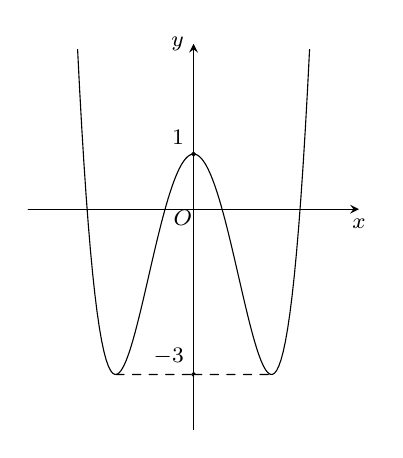
\begin{tikzpicture}[scale=0.7, font=\footnotesize, line join=round, line cap=round, >=stealth]
		\def\a{1} \def\b{-4} \def\c{1}
		\def\xmin{-3} \def\xmax{3}
		\def\ymin{-4} \def\ymax{3}
		%	\draw[color=gray!50,dashed] (\xmin,\ymin) grid (\xmax,\ymax);
		\draw[->] (\xmin,0)--(\xmax,0) node [below]{$x$};
		\draw[->] (0,\ymin)--(0,\ymax) node [left]{$y$};
		\node at (0,0) [below left=-3pt]{$O$};
		\clip (\xmin+0.1,\ymin+0.1) rectangle (\xmax-0.2,\ymax-0.1);
		\draw[samples=200,domain=-4:4] plot(\x,{\a*(\x)^4+\b*(\x)^2+\c});
		\draw[dashed](-1.41,-3)--(0,-3)node[above left]{$-3$}circle(1pt)--(1.41,-3);
		\draw(0,1)node[above left]{$1$}circle(1pt);
		\end{tikzpicture}
	}
	\loigiai{
		Phương trình đã cho tương đương với $f(x)=-\dfrac{1}{2}$ đây là phương trình hoành độ giao điểm của đồ thị hàm số $y=f(x)$ và $y=-\dfrac{1}{2}$. Dựa vào đồ thị ta thấy phương trình có $4$ nghiệm phân biệt.	
	}
\end{ex}

\begin{ex}%[Dự án 12EX6-2023]%[Đề thi thử SGD Hà Nội 2023, Nguyễn Anh Quốc]%[2D2B6-1]
	Bất phương trình $\log_2(2x-3)<1$ có tập nghiệm là $(a;b)$. Giá trị của $a+b$ bằng
	\choice
	{\True $4$}
	{$5$}
	{$2$}
	{$3$}
	\loigiai{
		Điều kiện $2x-3>0\Leftrightarrow x>\dfrac{3}{2}$.\\
		Bất phương trình đã cho tương đương với $2x-3<2\Leftrightarrow 2x<5\Leftrightarrow x<\dfrac{5}{2}$.\\
		So với điều kiện tập nghiệm của bất phương trình là $S=\left(\dfrac{3}{2};\dfrac{5}{2}\right)$.\\
		Từ đó ta suy ra $a=\dfrac{3}{2}$ và $b=\dfrac{5}{2}$ nên $a+b=\dfrac{3+5}{2}=4$.	
	}
\end{ex}

\begin{ex}%[Dự án 12EX6-2023]%[Đề thi thử SGD Hà Nội 2023, Nguyễn Anh Quốc]%[2D1B2-1]
	Cho hàm số $y=f(x)$ có $f'(x)=x(x-1)$. Hàm số đã cho có số điểm cực trị là	
	\choice
	{$1$}
	{$0$}
	{$3$}
	{\True $2$}
	\loigiai{
		Cho $f'(x)=0\Leftrightarrow x(x-1)=0\Leftrightarrow \hoac{&x=0\\&x=1.}$\\
		Phương trình $f'(x)=0$ có $2$ nghiệm đơn, nên hàm số $y=f(x)$ có $2$ điểm cực trị.	
	}
\end{ex}

\begin{ex}%[Dự án 12EX6-2023]%[Đề thi thử SGD Hà Nội 2023, Nguyễn Anh Quốc]%[2D2B5-2]
	Nghiệm của phương trình $2^{2x-1}=2^x$ là	
	\choice
	{$x=-2$}
	{$x=2$}
	{\True $x=1$}
	{$x=-1$}
	\loigiai{
		Ta có
		$$2^{2x-1}=2^x\Leftrightarrow 2x-1=x\Leftrightarrow x=1.$$	
		Vậy nghiệm của phương trình là $x=1$.
	}
\end{ex}

\begin{ex}%[Dự án 12EX6-2023]%[Đề thi thử SGD Hà Nội 2023, Nguyễn Anh Quốc]%[2D2B5-2]
	Tập nghiệm của phương trình $\log_3(x-3)=\log_3(2x-1)$ là
	\choice
	{$\{-2\}$}
	{$\{0\}$}
	{$\{2\}$}
	{\True $\varnothing$}
	\loigiai{
		Ta có $$\log_3(x-3)=\log_3(2x-1)\Leftrightarrow \heva{&x-3>0\\&x-3=2x-1}\Leftrightarrow \heva{&x>3\\&x=-2\text{ (loại)}.}$$	
		Phương trình đã cho vô nghiệm.
	}
\end{ex}

\begin{ex}%[Dự án 12EX6-2023]%[Đề thi thử SGD Hà Nội 2023, Nguyễn Anh Quốc]%[2D2B3-2]
	Với $a$, $b$ là các số thực dương, tùy ý $\log\left(a^2b^3\right)$ bằng	
	\choice
	{$6\log(ab)$}
	{$2\log a+\dfrac{1}{3}\log b$}
	{$\dfrac{1}{2}\log a+\dfrac{1}{3}\log b$}
	{\True $2\log a+3\log b$}
	\loigiai{
		Ta có  $\log\left(a^2b^3\right)=\log a^2+\log b^3=2\log a+3\log b.$	
	}
\end{ex}

\begin{ex}%[Dự án 12EX6-2023]%[Đề thi thử SGD Hà Nội 2023, Nguyễn Anh Quốc]%[2H1B3-2]
	Cho hình chóp tứ giác $S.ABCD$ có đáy $ABCD$ là hình vuông bằng $a\sqrt{3}$, $SA=a\sqrt{6}$ và $SA$ vuông góc với mặt đáy. Thể tích khối chóp $S.ABCD$ bằng	
	\choice
	{$\dfrac{a^3\sqrt{6}}{2}$}
	{$\dfrac{a^3\sqrt{6}}{3}$}
	{$a^3\sqrt{3}$}
	{\True $a^3\sqrt{6}$}
	\loigiai{
		\immini{
			Diện tích hình vuông $ABCD$ là $S=\left(a\sqrt{3}\right)^2=3a^2.$\\
			Thể tích khối chóp $S.ABCD$ là $V=\dfrac{1}{3}\cdot a\sqrt{6}\cdot 3a^2= a^3\sqrt{6}$.	
		}
		{\begin{tikzpicture}[scale=0.7,>=stealth, font=\footnotesize, line join=round, line cap=round]
			\tkzDefPoints{0/0/A,-1.3/-1.6/B,2.5/-1.6/C}
			\coordinate (D) at ($(A)+(C)-(B)$);
			\coordinate (S) at ($(A)+(0,3)$);
			\tkzDrawPolygon(S,B,C,D)
			\tkzDrawSegments(S,C)
			\tkzDrawSegments[dashed](A,S A,B A,D)
			\tkzDrawPoints[fill=black](D,C,A,B,S)
			\tkzMarkRightAngles[size=0.16](S,A,B S,A,D)
			\tkzLabelPoints[above](S)
			\tkzLabelPoints[below](A,B,C)
			\tkzLabelPoints[right](D)
			\end{tikzpicture}}	
	}
\end{ex}

\begin{ex}%[Dự án 12EX6-2023]%[Đề thi thử SGD Hà Nội 2023, Nguyễn Anh Quốc]%[2D3B2-2]
	Cho $I=\displaystyle\int ^2_1 2x \sqrt{x^2-1}\mathrm{\,d}x$. Nếu đặt $u=x^2-1$ thì khẳng định nào sau đây  đúng?	
	\choice
	{$I=\dfrac{1}{2}\displaystyle\int^3_0\sqrt{u}\mathrm{\,d}u$}
	{$I=\displaystyle\int^2_0\sqrt{u}\mathrm{\,d}u$}
	{\True $I=\displaystyle\int^3_0\sqrt{u}\mathrm{\,d}u$}
	{$I=2\displaystyle\int^3_0\sqrt{u}\mathrm{\,d}u$}
	\loigiai{
		Đặt $u=x^2-1\Rightarrow \mathrm{d}u=2x\mathrm{\,d}x$.\\
		Đổi cận $\heva{&x=1\Rightarrow u=0\\&x=2\Rightarrow u=3.}$\\
		Khi đó $I=\displaystyle\int^3_0\sqrt{u}\mathrm{\,d}u$.	
	}
\end{ex}

\begin{ex}%[Dự án 12EX6-2023]%[Đề thi thử SGD Hà Nội 2023, Nguyễn Anh Quốc]%[1D3B4-3]
	Cho cấp số nhân $\left(u_n\right)$ với $u_1=5$, $u_6=160$. Công bội của cấp số nhân bằng	
	\choice
	{$31$}
	{\True $2$}
	{$32$}
	{$5$}
	\loigiai{
		Ta có $u_6=u_1q^5\Rightarrow 160=5q^5\Rightarrow 32=q^5\Rightarrow q=2$.	
	}
\end{ex}

\begin{ex}%[Dự án 12EX6-2023]%[Đề thi thử SGD Hà Nội 2023, Nguyễn Anh Quốc]%[2H3B1-3]
	Trong KG $Oxyz$, mặt cầu $(S)\colon x^2+y^2+z^2-8x+4y+2z-4=0$ có bán kính bằng	
	\choice
	{$\sqrt{5}$}
	{$25$}
	{$2$}
	{\True $5$}
	\loigiai{
		Ta có $a=4$, $b=-2$, $c=-1$, $d=-4$.\\
		Ta suy ra $R=\sqrt{a^2+b^2+c^2-d}=\sqrt{16+4+1+4}=5$.	
	}
\end{ex}

\begin{ex}%[Dự án 12EX6-2023]%[Đề thi thử SGD Hà Nội 2023, Nguyễn Anh Quốc]%[2D3B3-3]
	Cho hình phẳng $(H)$ giới hạn bởi các đường $y=x^2-4$ và $y=0$. Thể tích khối tròn xoay được sinh bởi hình $(H)$ quay quanh trục $Ox$ có giá trị bằng	
	\choice
	{$\dfrac{256\pi}{15}$}
	{\True $\dfrac{512 \pi}{15}$}
	{$\dfrac{128 \pi}{5}$}
	{$\dfrac{512}{15}$}
	\loigiai{
		Xét phương trình $x^2-4=0\Leftrightarrow \hoac{&x=2\\&x=-2.}$\\
		Thể tích khối tròn xoay là 
		$$V=\pi \displaystyle\int^2_{-2}\left(x^2-4\right)^2\mathrm{\,d}x=\dfrac{512\pi }{15}.$$	
	}
\end{ex}

\begin{ex}%[Dự án 12EX6-2023]%[Đề thi thử SGD Hà Nội 2023, Nguyễn Anh Quốc]%[1H3B4-3]
	Cho hình lăng trụ đứng $ABC.A'B'C'$ có đáy $ABC$ là tam giác vuông cân tại $B$ có $AB=a$, $AA'=a\sqrt{2}$. Góc giữa đường thẳng $A'C$ và mặt phẳng $\left(AA'B'B\right)$ bằng	
	\choice
	{$60^\circ$}
	{\True $30^\circ$}
	{$90^\circ$}
	{$45^\circ$}
	\loigiai{
		\immini{
			Ta có $BC\perp AB$ và $BB'\perp BC$ nên $BC\perp (ABB'A')$.\\
			Suy ra góc giữa $A'C$ và $(ABB'A')$ là góc $CA'B$.\\
			Ta có $A'B=\sqrt{AB^2+AA'^2}=\sqrt{a^2 +2a^2}=a\sqrt{3}$.\\
			Xét tam giác vuông $A'BC$ ta có $\tan \widehat{CA'B}=\dfrac{BC}{A'B}=\dfrac{a}{a\sqrt{3}}=\dfrac{\sqrt{3}}{3}\Rightarrow \widehat{CA'B}=30^\circ$.
		}
		{\begin{tikzpicture}[scale=1,>=stealth, font=\footnotesize, line join=round, line cap=round]
			\tkzDefPoints{0/0/A,1.1/-1.5/B,3.5/0/C}
			\coordinate (A') at ($(A)+(0,3.2)$);
			\tkzDefPointsBy[translation=from A to A'](B,C){B'}{C'}
			\tkzDrawPolygon(A,B,C,C',B',A')
			\tkzDrawSegments(A',C' B',B A',B)
			\tkzDrawSegments[dashed](A,C A',C)
			\tkzDrawPoints[fill=black](A,C,B,A',B',C')
			\tkzLabelPoints[above](B')
			\tkzLabelPoints[below](B)
			\tkzLabelPoints[left](A',A)
			\tkzLabelPoints[right](C',C)
			\end{tikzpicture}}	
	}
\end{ex}

\begin{ex}%[Dự án 12EX6-2023]%[Đề thi thử SGD Hà Nội 2023, Nguyễn Anh Quốc]%[2D2B3-2]
	Cho $\log_3a=2$ và $\log_2b=\dfrac{1}{2}$. Khi đó $\log_3(3a)+\log_2b^2$ bằng
	\choice
	{\True $4$}
	{$0$}
	{$\dfrac{3}{2}$}
	{$\dfrac{5}{4}$}
	\loigiai{
		Ta có $\log_3(3a)+\log_2b^2=1+\log_3a+2\log_2b=1+2+2\cdot \dfrac{1}{2}=4.$	
	}
\end{ex}

\begin{ex}%[Dự án 12EX6-2023]%[Đề thi thử SGD Hà Nội 2023, Nguyễn Anh Quốc]%[2H3B2-7]
	Trong hông gian $Oxyz$, cho mặt phẳng $(\alpha)\colon (m+1)x+(m-1)y+6z-4=0$ và $(\beta)\colon 2x+y+3z-3=0$. Giá trị của tham số $m$ để hai mặt phẳng song song bằng	
	\choice
	{$2$}
	{$1$}
	{\True $3$}
	{$-1$}
	\loigiai{
		Ta có $(\alpha)\parallel (\beta)\Leftrightarrow \dfrac{m+1}{2}=\dfrac{m-1}{1}=\dfrac{6}{3}\ne \dfrac{-4}{-3}\Rightarrow \heva{&m+1=4\\&m-1=2}\Rightarrow m=3. $	
	}
\end{ex}

\begin{ex}%[Dự án 12EX6-2023]%[Đề thi thử SGD Hà Nội 2023, Nguyễn Anh Quốc]%[2D1B2-2]
	\immini{Cho hàm số bậc bốn $f(x)$. Hàm số $y=f'(x)$ có đồ thị như hình vẽ bên. Số điểm cực đại của hàm số $f(x)$ là
		\choice
		{\True $2$}
		{$3$}
		{$1$}
		{$0$}}
	{
		\begin{tikzpicture}[scale=1,>=stealth, font=\footnotesize, line join=round, line cap=round]
		%\def\a{1} \def\b{-6} \def\c{9} \def\d{1} % Hệ số
		\def\xmin{-1} \def\xmax{4}
		\def\ymin{-2} \def\ymax{3} 
		%\draw[color=gray!50,dashed] (\xmin,\ymin) grid (\xmax,\ymax); 
		\draw[->] (\xmin,0)--(\xmax,0) node [below]{$x$};
		\draw[->] (0,\ymin)--(0,\ymax) node [left]{$y$};
		\node at (0,0) [below left]{$O$};
		\clip (\xmin+0.1,\ymin+0.1) rectangle (\xmax-0.5,\ymax-0.1);
		\draw[smooth,samples=300,domain=-1:4] plot(\x,{-(\x-0.5)*(\x-1.5)*(\x-3)});
		\end{tikzpicture}
	}
	\loigiai{
		Ta thấy đồ thị hàm số $y=f'(x)$ cắt trục hoành tại ba điểm giả sử là $a$, $b$, $c$ với $(a<b<c)$. Khi đó ta có bảng biến thiên của hàm số $f(x)$ như sau
		\begin{center}
			
\begin{tikzpicture}
			\tkzTabInit[nocadre=false,lgt=1.2,espcl=2.5,deltacl=0.6]
			{$x$ /0.6,$f'(x)$ /0.6,$f(x)$ /2}
			{$-\infty$,$a$,$b$,$c$,$+\infty$}
			\tkzTabLine{,+,$0$,-,$0$,+,$0$,-,}
			\tkzTabVar{-/$-\infty$, +/$f(a)$,-/$f(b)$,+/$f(c)$,-/$-\infty$}
			\end{tikzpicture}
		\end{center}
		Vậy số điểm cực đại của hàm số $y=f(x)$ là $2$.	
	}
\end{ex}

\begin{ex}%[Dự án 12EX6-2023]%[Đề thi thử SGD Hà Nội 2023, Nguyễn Anh Quốc]%[1H3B5-3]
	Cho hình chóp $S.ABCD$ có đáy $ABCD$ là hình vuông cạnh bằng $a\sqrt{2}$, $SA=a\sqrt{3}$ và $SA$ vuông góc với mặt phẳng đáy. Khoảng cách từ $A$ đến mặt phẳng $(SBD)$ bằng	
	\choice
	{$a\sqrt{3}$}
	{$\dfrac{a\sqrt{30}}{5}$}
	{$a$}
	{\True $\dfrac{a\sqrt{3}}{2}$}
	\loigiai{
		\immini{
			Gọi $O$ là giao điểm của $AC$ và $BD$. Ta có $(SAC)\perp (SBD)$ và\\ $SO=(SAC)\cap (SBD)$. Kẻ $AH\perp SO$ khi đó $AH=\mathrm{d}(A,(SBD))$.\\
			Vì $ABCD$ là hình vuông nên $AC=2a$. Xét tam giác vuông $SAO$ ta có \\ $AH=\dfrac{AO\cdot SA}{\sqrt{AO^2+SA^2}}=\dfrac{a\cdot a\sqrt{3}}{\sqrt{a^2 +3a^2 }}=\dfrac{a\sqrt{3}}{2}.$
		}
		{\begin{tikzpicture}[scale=0.8,>=stealth, font=\footnotesize, line join=round, line cap=round]
			\tkzDefPoints{0/0/A,-1.3/-1.6/B,2.5/-1.6/C}
			\coordinate (D) at ($(A)+(C)-(B)$);
			\coordinate (S) at ($(A)+(0,3)$);
			\tkzInterLL(A,C)(B,D)\tkzGetPoint{O}
			\coordinate (H) at ($(S)!2/3!(O)$);
			\tkzDrawPolygon(S,B,C,D)
			\tkzDrawSegments(S,C)
			\tkzDrawSegments[dashed](A,S A,B A,D A,C B,D S,O A,H)
			\tkzDrawPoints[fill=black](D,C,A,B,S,O,H)
			\tkzMarkRightAngles[size=0.16](S,A,B S,A,D)
			\tkzLabelPoints[above](S)
			\tkzLabelPoints[below](A,B,C,O)
			\tkzLabelPoints[right](D,H)
			\end{tikzpicture}}	
	}
\end{ex}

\begin{ex}%[Dự án 12EX6-2023]%[Đề thi thử SGD Hà Nội 2023, Nguyễn Anh Quốc]%[2D1B3-1]
	Gọi $M$, $m$ lần lượt là giá trị lớn nhất và giá trị nhỏ nhất của hàm số $f(x)=x+\dfrac{4}{x}$ trên đoạn $[1;3]$. Khi đó tích $M$ và $m$ bằng	
	\choice
	{$15$}
	{$25$}
	{$6$}
	{\True $20$}
	\loigiai{
		Ta có $f'(x)=1-\dfrac{4}{x^2}=\dfrac{x^2-4}{x^2}$.\\
		$f'(x)=0\Leftrightarrow x^2-4=0\Leftrightarrow \hoac{&x=2\in [1;3]\\&x=-2\notin [1;3].}$\\
		Ta có $f(1)=5$, $f(2)=4$, $f(3)=\dfrac{13}{3}$.\\
		Giá trị lớn nhất và giá trị nhỏ nhất của hàm số $f(x)$ trên $[1;3]$ lần lượt là $M=5$, $m=4$.\\
		Vậy tích $M\cdot m=5\cdot 4=20$.	
	}
\end{ex}

\begin{ex}%[Dự án 12EX6-2023]%[Đề thi thử SGD Hà Nội 2023, Nguyễn Anh Quốc]%[1D2B5-2]
	Một hộp có $5$ viên bi đen và $4$ viên bi trắng. Lấy ngẫu nhiên $2$ viên bi trong hộp. Xác suất để lấy được $2$ viên bi cùng màu bằng	
	\choice
	{\True $\dfrac{4}{9}$}
	{$\dfrac{1}{9}$}
	{$\dfrac{5}{9}$}
	{$\dfrac{1}{4}$}
	\loigiai{
		Gọi $\Omega$ là không gian mẫu.\\
		Ta có $n(\Omega)=\mathrm{C}^2_9=36$.\\
		Gọi $A\colon$\lq\lq  lấy được hai viên bi cùng màu\rq\rq.\\
		Ta có $n(A)=\mathrm{C}^2_5+\mathrm{C}^2_4=10+6=16$.\\
		Xác suất của biến cố $A$ là $P(A)=\dfrac{n(A)}{n(\Omega)}=\dfrac{16}{36}=\dfrac{4}{9}$.
	}
\end{ex}

\begin{ex}%[Dự án 12EX6-2023]%[Đề thi thử SGD Hà Nội 2023, Nguyễn Anh Quốc]%[2H3B2-3]
	Trong KG $Oxyz$, cho $A(1;1;-1)$, $B(5;2;1)$. Phương trình mặt phẳng trung trực của đoạn $AB$ là	
	\choice
	{$8x+2y+4z+27=0$}
	{\True $8x+2y+4z-27=0$}
	{$6x+2y-21=0$}
	{$4x+y+2z-3=0$}
	\loigiai{
		Gọi $M$ là trung điểm của $AB$ khi đó $M\left(3;\dfrac{3}{2};0\right)$.\\
		Mặt phẳng trung trực của đoạn $AB$ đi qua $M$ và nhận $\overrightarrow{AB}=(4;1;2)$ là véc-tơ pháp tuyến.\\
		Phương trình tổng quát của mặt phẳng trung trực cần tìm là 
		$$4(x-3)+1\left(y-\dfrac{3}{2}\right)+2z=0\Leftrightarrow 4x+y+2z-\dfrac{27}{2}=0\Leftrightarrow 8x+2y+4z-27=0.$$
	}
\end{ex}

\begin{ex}%[Dự án 12EX6-2023]%[Đề thi thử SGD Hà Nội 2023, Nguyễn Anh Quốc]%[2H3K1-1]
	Trong KG $Oxyz$, cho tam giác $OAB$ có $A(2;2;-1)$ và $B(0;-4;3)$. Độ dài đường phân giác trong $\widehat{AOB}$ bằng	
	\choice
	{$\dfrac{\sqrt{30}}{5}$}
	{\True $\dfrac{\sqrt{30}}{4}$}
	{$\dfrac{9}{8}$}
	{$\dfrac{15}{8}$}
	\loigiai{
		
		\immini{
			Gọi $M(x;y;z)$ là chân đường phân giác trong $\widehat{AOB}$ khi đó ta có \\
			$\dfrac{MA}{MB}=\dfrac{OA}{OB}\Rightarrow \overrightarrow{MA}=-\dfrac{OA}{OB}\overrightarrow{MB}.$\\
			Mà $OA=\sqrt{4+4+1}=3$, $OB=\sqrt{16+9}=5$.\\
			Suy ra $\overrightarrow{MA}=-\dfrac{3}{5}\overrightarrow{MB}$\quad (1).\\
			Ta có $\overrightarrow{MA}=(2-x;2-y;-1-z)$, $\overrightarrow{MB}=(-x;-4-y;3-z)$.\\
			Từ $(1)$ suy ra $\heva{&2-x=\dfrac{3}{5}x\\&2-y=\dfrac{12+3y}{5}\\&-1-z=\dfrac{-9+3z}{5}}\Rightarrow \heva{&x=\dfrac{5}{4}\\&y=-\dfrac{1}{4}\\&z=\dfrac{1}{2}}\Rightarrow M\left(\dfrac{5}{4};-\dfrac{1}{4};\dfrac{1}{2}\right)$.\\
			Ta có $OM=\sqrt{\dfrac{25}{16}+\dfrac{1}{16}+\dfrac{1}{4}}=\dfrac{\sqrt{30}}{4}.$
		}
		{\begin{tikzpicture}[scale=0.8,>=stealth, font=\footnotesize, line join=round, line cap=round]
			\def\xmin{-1} \def\xmax{5}  \def\ymin{-1}  \def\ymax{4} 
			%	\draw[color=gray!50,dashed] (\xmin,\ymin) grid (\xmax,\ymax);
			%	\draw[->] (\xmin,0)--(\xmax,0) node [below]{$x$};
			%	\draw[->] (0,\ymin)--(0,\ymax) node [left]{$y$};
			\clip (\xmin,\ymin) rectangle (\xmax,\ymax);
			%%%%
			\tkzDefPoints{0/0/O,4/0/B,2/3/A}
			\tkzDrawBisector(A,O,B)\tkzGetPoint{M}
			\tkzDrawSegments(A,B O,A O,B)
			\tkzDrawPoints[fill=black](A,B,O,M)
			\tkzLabelPoints[below](B,O)
			\tkzLabelPoints[above](A)
			\tkzLabelPoints[right](M)
			\end{tikzpicture}}	
	}
\end{ex}

\begin{ex}%[Dự án 12EX6-2023]%[Đề thi thử SGD Hà Nội 2023, Nguyễn Anh Quốc]%[2D1K2-6]
	\immini{Cho hàm số bậc bốn $y=f(x)$ có đồ thị như hình vẽ bên. Số giá trị nguyên dương của tham số $m$ để hàm số $g(x)=\left(f(x)+m\right)^2$ có $5$ điểm cực trị là	
		\choice
		{$3$}
		{$5$}
		{\True $4$}
		{$6$}}
	{\begin{tikzpicture}[scale=0.7,>=stealth, font=\footnotesize, line join=round, line cap=round]
		\def\xmin{-3} \def\xmax{5}
		\def\ymin{-7} \def\ymax{2} 
		%\draw[color=gray!50,dashed] (\xmin,\ymin) grid (\xmax,\ymax); 
		\draw[->] (\xmin,0)--(\xmax,0) node [below]{$x$};
		\draw[->] (0,\ymin)--(0,\ymax) node [left]{$y$};
		\node at (0,0) [below left]{$O$};
		\clip (\xmin+0.1,\ymin+0.1) rectangle (\xmax-0.5,\ymax-0.1);
		\draw plot[smooth,tension=0.7]coordinates{(-2,2) (-1,-4) (1,-2) (3,-6) (4,2)};
		\draw[dashed] (0,-1.95)node[left]{$-2$}circle(1pt)--(0.9,-1.95) (-0.9,-4.1)--(0,-4.1)node[right]{$-4$}circle(1pt) (0,-6.1)node[left]{$-6$}circle(1pt)--(2.9,-6.1);
		\end{tikzpicture}}
	\loigiai{
		Ta có $g'(x)=2\left(f(x)+m\right)f'(x)$.\\
		Ta thấy $g'(x)=0\Leftrightarrow \hoac{&f'(x)=0\quad (1)\\&f(x)+m=0.\quad (2)}$\\
		Xét phương trình $(1)$, dựa vào đồ thị hàm số $f(x)$ thấy hàm số có ba điểm cực trị nên phương trình $f'(x)=0$ có $3$ nghiệm đơn.\\
		Do đó để hàm số $g(x)$ có $5$ điểm cực trị khi và chỉ khi $(2)$ có $2$ nghiệm bội lẻ. \\Dựa vào đồ thị ta thấy  $\hoac{&-m\ge -2\\&-6<-m\le -4}\Leftrightarrow \hoac{&m\le 2\\&4\le m<6.}$\\
		Vì $m$ là số nguyên dương nên $m\in\{1;2;4;5\}$.
	}
\end{ex}

\begin{ex}%[Dự án 12EX6-2023]%[Đề thi thử SGD Hà Nội 2023, Nguyễn Anh Quốc]%[2D2K5-3]
	Gọi $S$ là tập hợp tất cả các giá trị nguyên của tham số $m$ để phương trình $4^x-2^{x+2}-m=0$ có đúng hai nghiệm phân biệt. Tích các phần tử của $S$ bằng	
	\choice
	{\True $-6$}
	{$-12$}
	{$6$}
	{$0$}
	\loigiai{
		Đặt $t=2^x$ với $t>0$. Khi đó phương trình đã cho trở thành $t^2-4t-m=0$\quad (1).\\
		Phương trình đã cho có hai nghiệm phân biệt khi và chỉ khi phương trình $(1)$ có hai nghiệm dương phân biệt hay $$\heva{&\Delta'>0\\&S>0\\&P>0}\Leftrightarrow \heva{&4+m>0\\&4>0\\&-m>0}\Leftrightarrow -4<m<0.$$
		Vì $m$ là số nguyên nên $m\in \{-3;-2;-1\}$.\\
		Suy ra tích $-3\cdot (-2)\cdot (-1)=-6$.
	}
\end{ex}

\begin{ex}%[Dự án 12EX6-2023]%[Đề thi thử SGD Hà Nội 2023, Nguyễn Anh Quốc]%[2D1K5-5]
	\immini{Cho hàm số bậc năm $f(x)$. Hàm số $y=f'(x)$ có đồ thị như hình vẽ bên. Số điểm cực trị của hàm số $g(x)=f(x)+\dfrac{2}{3}x^3-2x^2+3x$ là	
		\choice
		{\True $0$}
		{$1$}
		{$3$}
		{$2$}}
	{\begin{tikzpicture}[scale=0.7,>=stealth, font=\footnotesize, line join=round, line cap=round]
		\def\xmin{-3} \def\xmax{3}
		\def\ymin{-2} \def\ymax{5} 
		%	\draw[color=gray!50,dashed] (\xmin,\ymin) grid (\xmax,\ymax); 
		\draw[->] (\xmin,0)--(\xmax,0) node [below]{$x$};
		\draw[->] (0,\ymin)--(0,\ymax) node [left]{$y$};
		\node at (0,0) [below left]{$O$};
		\clip (\xmin+0.1,\ymin+0.1) rectangle (\xmax-0.5,\ymax-0.1);
		\draw plot[smooth,tension=0.7]coordinates{(-2,4) (-1.5,1.5) (0,2) (1,-1) (2,4)};
		\draw[dashed] (0,2)node[below left]{$2$}circle(1pt) (0,-1)node[left]{$-1$}circle(1pt)--(1,-1)--(1,0)node[above]{$1$}circle(1pt);
		\end{tikzpicture}}
	\loigiai{
		\immini{Ta có $g'(x)=f'(x)+2x^2-4x+3$, $g'(x)=0\Leftrightarrow f'(x)=-2x^2+4x-3$. Đây là phương trình hoành độ giao điểm của đồ thị hàm số $y=f'(x)$ và $y=-2x^2+4x-3$.\\
			Dựa vào đồ thị ta thấy $f'(x)$ và $y=-2x^2+4x-3$ tiếp xúc nhau tại $x=1$ nên phương trình $g'(x)=0$ chỉ có nghiệm bội chẵn. Do đó, hàm số $g(x)$ không có điểm cực trị.}
		{\begin{tikzpicture}[scale=0.7,>=stealth, font=\footnotesize, line join=round, line cap=round]
			\def\xmin{-3} \def\xmax{4}
			\def\ymin{-4} \def\ymax{5} 
			%	\draw[color=gray!50,dashed] (\xmin,\ymin) grid (\xmax,\ymax); 
			\draw[->] (\xmin,0)--(\xmax,0) node [below]{$x$};
			\draw[->] (0,\ymin)--(0,\ymax) node [left]{$y$};
			\node at (0,0) [below left]{$O$};
			\clip (\xmin+0.1,\ymin+0.1) rectangle (\xmax-0.5,\ymax-0.1);
			\draw plot[smooth,tension=0.7]coordinates{(-2,4) (-1.5,1.5) (0,2) (1,-1) (2,4)};
			\draw[dashed] (0,2)node[below left]{$2$}circle(1pt) (0,-1)node[left]{$-1$}circle(1pt)--(1,-1)--(1,0)node[above]{$1$}circle(1pt);
			\draw[smooth,domain=-3:3]plot(\x,{-2*(\x)^2+4*(\x)-3});
			\end{tikzpicture}}	
	}
\end{ex}

\begin{ex}%[Dự án 12EX6-2023]%[Đề thi thử SGD Hà Nội 2023, Nguyễn Anh Quốc]%[2H2B2-6]
	\immini{Một xe bồn chở nước có bồn nước gồm hai nửa hình cầu đường kính $18$ dm	 và một hình trụ có chiều cao $36$ dm (như hình vẽ). Thể tích của khối bồn đã cho bằng
		\choice
		{$9216\pi$ dm$^3$}
		{$\dfrac{1024\pi}{9}$ dm$^3$}
		{\True $3888\pi$ dm$^3$}
		{$\dfrac{16\pi}{243}$ dm$^3$}}
	{\begin{tikzpicture}[scale=0.8,>=stealth, font=\footnotesize, line join=round, line cap=round]
		\def\xmin{-5.5} \def\xmax{5.5}  \def\ymin{-1.5}  \def\ymax{2.5} 
		\def\d{3} \def\r{1}
		%	\draw[color=gray!50,dashed] (\xmin,\ymin) grid (\xmax,\ymax);
		%	\draw[->] (\xmin,0)--(\xmax,0) node [below]{$x$};
		%	\draw[->] (0,\ymin)--(0,\ymax) node [left]{$y$};
		\clip (\xmin,\ymin) rectangle (\xmax,\ymax);
		%%%%
		
		\tkzDefPoints{0/0/O,4/0/A,-4/0/B,-4/\r/I,4/\r/J}
		\tkzDrawArc[R](I,\r cm)(90,270)
		\tkzDrawArc[R](J,\r cm)(-90,90)
		\draw[rotate=-90] (B) arc (0:180:1cm and 0.6cm);
		\draw[rotate=-90,dashed] (B) arc (0:-180:1cm and 0.6cm);
		\draw[rotate=-90] (A) arc (0:180:1cm and 0.6cm);
		\draw[rotate=-90,dashed] (A) arc (0:-180:1cm and 0.6cm);
		\draw[dashed](B)--(-4,2) (4,2)--(A);
		\draw (A)--(B) (-4,2)--(4,2);
		\draw[<->,dashed](0,0)--(0,2);
		\draw (0,1)node[right]{$18$ dm}; \draw[<->](-4,-0.5)--(0,-0.5)node[below]{$36$ dm}--(4,-0.5);
		\end{tikzpicture}}
	\loigiai{
		Thể tích của hai nửa khối cầu là $V_1=\dfrac{4}{3}\pi \cdot 9^3=972\pi$ dm$^3$.\\
		Thể tích phần khối trụ là $V_2=\pi\cdot 9^2\cdot 36=2916\pi $ dm$^3$.\\
		Vậy thể tích của bồn là $V=V_1+V_2=972\pi +2916\pi =3888\pi$ dm$^3$.	
	}
\end{ex}

\begin{ex}%[Dự án 12EX6-2023]%[Đề thi thử SGD Hà Nội 2023, Nguyễn Anh Quốc]%[2D1K5-7]
	Cho hàm số $f(x)=x^3-3x$. Số hình vuông có bốn đỉnh nằm trên đồ thị của hàm số $y=f(x)$ là	
	\choice
	{\True $2$}
	{$4$}
	{$3$}
	{$1$}
	\loigiai{
		Đồ thị $(C)$ của hàm số $f(x)$ có tâm đối xứng là gốc tọa độ nên hình vuông có bốn điểm nằm trên đồ thị cũng có tâm đối xứng là gốc tọa độ. Giả sử hình vuông cần tìm là $ABCD$, khi đó $AC\colon y=ax$ và $BD\colon y=-\dfrac{1}{a}x$ với $a\ne 0$.
		\begin{itemize}
			\item Tìm tọa độ giao điểm của $AC$ với $(C)$.\\
			Xét phương trình $x^3-3x=ax\Leftrightarrow x\left(x^2-3-a\right)=0\Leftrightarrow \hoac{&x=0\\&x=\pm \sqrt{3+a} \text{ với }a>-3.}$\\
			Giả sử $A\left(\sqrt{3+a};a\sqrt{3+a}\right)$, $C\left(-\sqrt{3+a};-a\sqrt{3+a}\right)$.
			\item Tìm tọa độ giao điểm của $BD$ với $(C)$.\\
			Xét phương trình $x^3-3x=-\dfrac{1}{a}x\Leftrightarrow x\left(x^2-3+\dfrac{1}{a}\right)=0\Leftrightarrow \hoac{&x=0\\&x=\pm \sqrt{3-\dfrac{1}{a}}\text{ với }a<0 \text{ hoặc }a> \dfrac{1}{3}.}$\\
			Giả sử $B\left(\sqrt{\dfrac{3a-1}{a}};-\dfrac{1}{a}\cdot\sqrt{\dfrac{3a-1}{a}}\right)$ và $D\left(-\sqrt{\dfrac{3a-1}{a}};\dfrac{1}{a}\cdot\sqrt{\dfrac{3a-1}{a}}\right)$.
		\end{itemize}
		Ta có 
		\begin{eqnarray*}
			&&AC=BD\Leftrightarrow OA=OB\\
			&\Leftrightarrow& \sqrt{3+a+a^2(3+a)}=\sqrt{\dfrac{3a-1}{a}+\dfrac{1}{a^2}\cdot \dfrac{3a-1}{a}}\\
			&\Leftrightarrow&(3+a)\left(a^2+1\right)=\dfrac{3a-1}{a}\left(\dfrac{a^2+1}{a^2}\right)\\
			&\Leftrightarrow&(3+a)a^3=3a-1\Leftrightarrow a^4+3a^3-3a+1=0\\
			&\Leftrightarrow&\left(a^2+2a-1\right)\left(a^2+a-1\right)=0\Leftrightarrow \hoac{&a^2+2a-1=0\\&a^2+a-1=0}\\
		&\Leftrightarrow&\hoac{&a=-1\pm \sqrt{2}\\&a=\dfrac{-1\pm\sqrt{5}}{2}.}	\end{eqnarray*}
		Ta thấy điều kiện tổng hợp là $a\in (-3;0)\cup \left(\dfrac{1}{3};+\infty\right)$ và các giá trị $a=-1\pm \sqrt{2}$, $a=\dfrac{-1\pm\sqrt{5}}{2}$ đều thỏa mãn.\\
		Mặt khác,  $-\dfrac{1}{-1\pm \sqrt{2}}=-1\mp \sqrt{2}$ và $-\dfrac{1}{\dfrac{-1\pm \sqrt{5}}{2}}=\dfrac{-1\mp \sqrt{5}}{2}$. Nên ta chọn hai giá trị của $a$ là  $-1+\sqrt{2}$ và $\dfrac{-1+\sqrt{5}}{2}$.
	}
\end{ex}

\begin{ex}%[Dự án 12EX6-2023]%[Đề thi thử SGD Hà Nội 2023, Nguyễn Anh Quốc]%[2D3K3-1]
	\immini{Cho	hai hàm số bậc bốn $f(x)$, $g(x)$ có đồ thị $y=f'(x)$ và $y=g'(x)$ như hình vẽ. Số giá trị thực của tham số $m$ để phương trình $f(x)-g(x)=m$ có một nghiệm duy nhất trên $[-1;3]$ là
		\choice
		{Vô số}
		{$0$}
		{$2$}
		{\True $1$}}
	{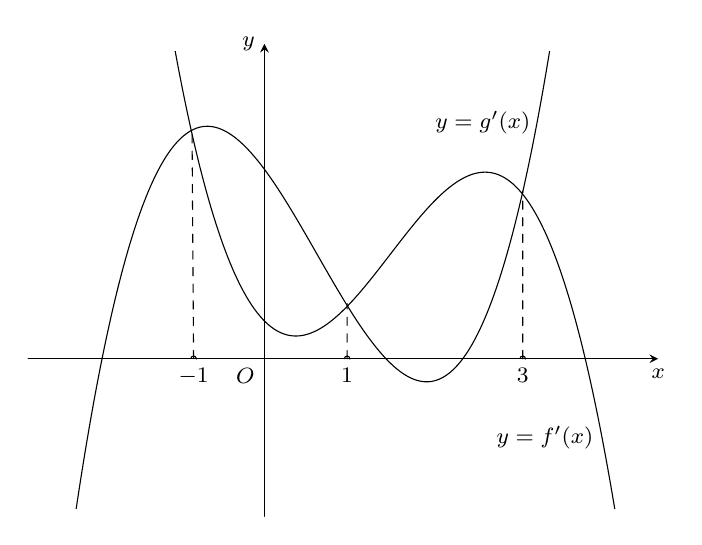
\begin{tikzpicture}[scale=1,>=stealth, font=\footnotesize, line join=round, line cap=round]
		\def\xmin{-3} \def\xmax{5}
		\def\ymin{-2} \def\ymax{4} 
		%	\draw[color=gray!50,dashed] (\xmin,\ymin) grid (\xmax,\ymax); 
		\draw[->] (\xmin,0)--(\xmax,0) node [below]{$x$};
		\draw[->] (0,\ymin)--(0,\ymax) node [left]{$y$};
		\node at (0,0) [below left]{$O$};
		\clip (\xmin+0.1,\ymin+0.1) rectangle (\xmax-0.5,\ymax-0.1);
		\draw[smooth,samples=300] plot(\x,{-0.3*(\x-4)*(\x-0.5)*(\x-0.3)+0.3});
		\draw[smooth,samples=300] plot(\x,{0.3*(\x+2)*(\x-1.3)*(\x-2.7)+0.3});
		\draw[dashed](-0.9,0)node[below]{$-1$}circle(1pt)--(-0.92,2.95) (1.05,0)node[below]{$1$}circle(1pt)--(1.05,0.7) (3.28,0)node[below]{$3$}circle(1pt)--(3.28,2.13);
		\draw (3.5,3)node[left]{$y=g'(x)$} (4.3,-1)node[left]{$y=f'(x)$}; 
		\end{tikzpicture}}
	\loigiai{
		Đặt $h(x)=f(x)-g(x)$, ta có $h'(x)=f'(x)-g'(x)=a(x+1)(x-1)(x-3)$.\\
		Ta có bảng biến thiên của hàm số $h(x)$ như sau
		\begin{center}
			
\begin{tikzpicture}
			\tkzTabInit[nocadre=false,lgt=1.2,espcl=2.5,deltacl=0.6]
			{$x$ /0.6,$h'(x)$ /0.6,$h(x)$ /2}
			{$-\infty$,$-1$,$1$,$3$,$+\infty$}
			\tkzTabLine{,+,$0$,-,$0$,+,$0$,-,}
			\tkzTabVar{-/$-\infty$, +/$h(-1)$,-/$h(1)$,+/$h(3)$,-/$-\infty$}
			\end{tikzpicture}
		\end{center}
		Dựa vào bảng xét dấu ta thấy hệ số $a<0$. \\
		Mặt khác ta thấy rằng $\displaystyle\int^1_{-1}\left|f'(x)-g'(x)\right|\mathrm{\,d}x=\displaystyle\int^1_{-1}\left|a(x+1)(x-1)(x-3)\right|\mathrm{\,d}x=4|a|$ và\\ $\displaystyle\int^3_1\left|f'(x)-g'(x)\right|\mathrm{\,d}x=\displaystyle\int^3_1\left|a(x+1)(x-1)(x-3)\right|\mathrm{\,d}x=4|a|$.\\
		Từ đó ta suy ra $\displaystyle\int ^1_{-1}\left[f'(x)-g'(x)\right]\mathrm{\,d}x=\displaystyle\int ^3_1\left[g'(x)-f'(x)\right]\mathrm{\,d}x\Leftrightarrow f(1)-g(1)-f(-1)+g(-1)=g(3)-f(3)-g(1)+f(1)$.\\
		Suy ra $f(3)-g(3)=f(-1)-g(-1)\Rightarrow h(3)=h(-1)$.\\
		Từ đó suy ra phương trình $f(x)-g(x)=m\Leftrightarrow h(x)=m$ có một nghiệm duy nhất trong $[-1;3]$ khi $m=h(1)$.\\
		Vậy có $1$ giá trị của tham số $m$ để phương trình $f(x)-g(x)=m$ có nghiệm duy nhất.
	}
\end{ex}

\begin{ex}%[Dự án 12EX6-2023]%[Đề thi thử SGD Hà Nội 2023, Nguyễn Anh Quốc]%[2H1G3-2]
	Cho hình chóp $S.ABC$ có đáy $ABC$ là tam giác vuông cân tại $A$, tam giác $SBA$ vuông tại $B$ và tam giác $SBC$ là tam giác đều cạnh $2a$. Thể tích khối chóp $S.ABC$ bằng	
	\choice
	{$\dfrac{a^3}{6}$}
	{$\dfrac{a^3\sqrt{3}}{3}$}
	{\True $\dfrac{a^3\sqrt{2}}{3}$}
	{$\dfrac{a^3}{3}$}
	\loigiai{
		\immini{
			Gọi $E$ là hình chiếu của $S$ lên $(ABC)$, vì $SAB$ là tam giác vuông tại $B$ nên $AB\perp (SBE)$. Mặt khác $ABC$ là tam giác vuông tại $A$ nên $AC\parallel BE$. Gọi $D$ thuộc $BE$ sao cho $ABDC$ hình bình hành. Vì $ABC$ là tam giác vuông cân nên $ABDC$ là hình vuông. Gọi $F$ là giao điểm của $AD$ và $BC$, vì $SBC$ là tam giác đều cạnh $2a$ nên $SF\perp BC$ và $SF=a\sqrt{3}$. Ta có cũng có $BC\perp SE$ nên $BC\perp (SEF)$ suy ra $BC\perp EF$. Từ đó suy ra $\triangle BFE$ và $\triangle BDC$ là hai tam giác vuông đồng dạng, ta suy ra $\dfrac{BE}{BC}=\dfrac{BF}{BD}\Rightarrow BE=\dfrac{BF\cdot BC}{BD}=\dfrac{a\cdot 2a }{a\sqrt{2}}=a\sqrt{2}.$\\
			Xét tam giác vuông $SEB$ ta có $SE=\sqrt{ SB^2-BE^2 }=\sqrt{ 4a^2 -2a^2 }=a\sqrt{ 2}$.\\
			Diện tích tam giác $ABC$ là $S_{ABC}=\dfrac{(a\sqrt{2})^2}{2}=a^2 $.\\
			Thể tích khối chóp $S.ABC$ là $V=\dfrac{1}{3}\cdot SE\cdot S_{ABC}=\dfrac{1}{3}\cdot a\sqrt{2}\cdot a^2 =\dfrac{a^3\sqrt{2}}{3}$.
			
		}
		{\begin{tikzpicture}[scale=0.8,>=stealth, font=\footnotesize, line join=round, line cap=round]
			\def\xmin{-1} \def\xmax{5}  \def\ymin{-3}  \def\ymax{3} 
			%	\draw[color=gray!50,dashed] (\xmin,\ymin) grid (\xmax,\ymax);
			%	\draw[->] (\xmin,0)--(\xmax,0) node [below]{$x$};
			%	\draw[->] (0,\ymin)--(0,\ymax) node [left]{$y$};
			\clip (\xmin,\ymin) rectangle (\xmax,\ymax);
			%%%%
			\tkzDefPoints{0/0/A,3/0/C,1.5/-2/B}
			\coordinate (D) at ($(B)+(C)-(A)$);
			\tkzInterLL(A,D)(B,C)\tkzGetPoint{F}
			\coordinate (E) at ($(D)!0.2!(B)$);
			\coordinate (S) at ($(E)+(0,4)$);
			\tkzDrawSegments(A,B S,A S,E S,D S,B B,D)
			\tkzDrawSegments[dashed](A,C B,C A,E S,F F,E C,D S,C)
			\tkzDrawPoints[fill=black](A,B,C,D,E,F,S)
			\tkzLabelPoints[below](B,C,D,E,F)
			\tkzLabelPoints[above](S)
			\tkzLabelPoints[left](A)
			\end{tikzpicture}}
	}
\end{ex}

\begin{ex}%[Dự án 12EX6-2023]%[Đề thi thử SGD Hà Nội 2023, Nguyễn Anh Quốc]%[2D3G2-2]
	Cho hàm số $y=f(x)$ có đạo hàm trên $(0;+\infty)$ thỏa mãn $f(1)=1$ và $\mathrm{e}^xf'\left(\mathrm{e}^x\right)=1+\mathrm{e}^x$. Khi đó $\displaystyle \int^\mathrm{e}_1f(x)\mathrm{\,d}x$ bằng
	\choice
	{$\dfrac{\mathrm{e}^2-1}{2}$}
	{$\dfrac{3\mathrm{e}^2-2}{2}$}
	{\True $\dfrac{\mathrm{e}^2+1}{2}$}
	{$\dfrac{\mathrm{e}^2}{2}$}
	\loigiai{
		Từ $\mathrm{e}^xf'\left(\mathrm{e}^x\right)=1+\mathrm{e}^x$. Lấy nguyên hàm hai vế ta được
		$$\displaystyle\int \mathrm{e}^xf'\left(\mathrm{e}^x\right)\mathrm{\,d}x=\displaystyle\int \left(1+\mathrm{e}^x\right)\mathrm{\,d}x\Rightarrow f\left(\mathrm{e}^x\right)=x+\mathrm{e}^x+C.$$
		Vì $f(1)=0+\mathrm{e}^0+C=1\Rightarrow C=0$.\\
		Suy ra $f\left(\mathrm{e}^x\right)=x+\mathrm{e}^x\Rightarrow f\left(\mathrm{e}^x\right)\mathrm{e}^x=x\mathrm{e}^x+\mathrm{e}^{2x}$.\\
		Lấy tích phân từ $0$ đến $1$ hai vế ta được
		$$I=\displaystyle\int^1_0 f\left(\mathrm{e}^x\right)\mathrm{e}^x\mathrm{\,d}x=\displaystyle\int^1_0\left(x\mathrm{e}^x+\mathrm{e}^{2x}\right)\mathrm{\,d}x.$$
		Xét $I=\displaystyle\int^1_0 f\left(\mathrm{e}^x\right)\mathrm{e}^x\mathrm{\,d}x$. Đặt $t=\mathrm{e}^x$ khi đó $I=\displaystyle \int^\mathrm{e}_1f(t)\mathrm{\,d}t$.\\
		Xét $I=\displaystyle\int^1_0\left(x\mathrm{e}^x+\mathrm{e}^{2x}\right)\mathrm{\,d}x=x\mathrm{e}^x\bigg|^1_0-\mathrm{e}^x\bigg|^1_0+\dfrac{1}{2}\mathrm{e}^{2x}\bigg|^1_0=\mathrm{e}-\mathrm{e}+1+\dfrac{1}{2}\mathrm{e}^2-\dfrac{1}{2}=\dfrac{\mathrm{e}^2+1}{2}.$\\
		Vậy $I=\dfrac{\mathrm{e}^2+1}{2}$.
	}
\end{ex}

\begin{ex}%[Dự án 12EX6-2023]%[Đề thi thử SGD Hà Nội 2023, Nguyễn Anh Quốc]%[2H3G2-8]
	Trong KG $Oxyz$, cho điểm $A(-2;6;0)$ và mặt phẳng $(\alpha)\colon 3x+4y+89=0$. Đường thẳng $d$ thay đổi nằm trên mặt phẳng $(Oxy)$ và luôn đi qua điểm $A$. Gọi $H$ là hình chiếu vuông góc của $M(4;-2;3)$ trên đường thẳng $d$. Khoảng cách nhỏ nhất từ $H$ đến mặt phẳng $(\alpha)$ bằng	
	\choice
	{\True $15$}
	{$90$}
	{$\dfrac{68}{5}$}
	{$\dfrac{93}{5}$}
	\loigiai{
		\immini{Vì $H$ thuộc $(Oxy)$ và $MH\perp AH$ nên $H$ thuộc đường tròn giao tuyến $(C)$ của  $(Oxy)$ và mặt cầu $(S)$ đường kính\\ $MA=\sqrt{6^2 +8^2 +3^2}=\sqrt{109}$. Gọi $I$ tâm mặt cầu $(S)$ khi đó $I\left(1;2;\dfrac{3}{2}\right)$. Ta có $J(1;2;0)$ là tâm đường tròn giao tuyến $(C)$ là hình chiếu của $I$ lên $(Oxy)$. Hơn nữa, ta thấy $(\alpha)\perp (Oxy)$, do đó khoảng cách ngắn nhất từ $H$ đến $(\alpha)$ bẳng $\mathrm{d}(J,(\alpha))-r$.\\
			Ta có $r=\sqrt{\dfrac{MA^2}{4}-\mathrm{d}^2(I,(Oxy))}=\sqrt{\dfrac{109}{4}-\dfrac{9}{4}}=5$ và \\$\mathrm{d}(J,(\alpha))=\dfrac{|3+8+89|}{\sqrt{9+16}}=\dfrac{100}{5}=20$.\\
			Vậy khoảng cách ngắn nhất từ $H$ đến $(\alpha)$ là $20-5=15$.}
		{\begin{tikzpicture}[scale=1,>=stealth, font=\footnotesize, line join=round, line cap=round]
			\def\xmin{-4} \def\xmax{3}  \def\ymin{-3}  \def\ymax{4} 
			%	\draw[color=gray!50,dashed] (\xmin,\ymin) grid (\xmax,\ymax);
			%	\draw[->] (\xmin,0)--(\xmax,0) node [below]{$x$};
			%	\draw[->] (0,\ymin)--(0,\ymax) node [left]{$y$};
			\clip (\xmin,\ymin) rectangle (\xmax,\ymax);
			
			\def \x{2} %bán kính trục lớn elip
			\def \y{0.7} %bán kính trục bé elip
			\coordinate (I) at (0,0);
			\coordinate (B) at (\x,0);
			\coordinate (A) at (-\x,0);
			\coordinate (J) at ($(0,-0.5*\x)+(0,0.05)$);
			\coordinate (H) at ($(J)+(180:\x*0.866 cm and \y*0.866 cm)$);
			\coordinate (T) at ($(J)+(-60:\x*0.866 cm and \y*0.866 cm)$);
			\coordinate (m) at ($(J)+(-\x-1.1,-\y)$);
			\coordinate (n) at ($(J)+(\x+0.1,-\y)$);
			\coordinate (p) at ($(J)+(\x+0.9,\y)$);
			\coordinate (q) at ($(m)+(p)-(n)$);
			\tkzInterLC(p,q)(I,A)\tkzGetPoints{p'}{q'}
			\tkzInterLC(m,n)(I,A)\tkzGetPoints{x}{y}
			\draw (-34:\x) arc (-34:214:\x);
			\draw (y) arc (-124:-56:\x);
			\draw (x)[dashed] arc (-56:-30:\x);
			\draw (y)[dashed] arc (-124:-150:\x);
			\draw[dashed] ($(-30:\x)+(0,0.05)$) arc (0:180:\x*0.866 cm and \y*0.866 cm);
			\draw ($(-30:\x)+(0,0.05)$) arc (0:-180:\x*0.866 cm and \y*0.866 cm);
			\draw[dashed] (p')--(q') (I)--(J) (I)--(H) (J)--(H);
			\tkzDrawSegments(q',q q,m m,n n,p p,p')
			\tkzDrawPoints[fill=black](I,J,H)
			\tkzLabelPoints[above](I,H)
			\tkzLabelPoints[below](J)
			%\node at ($(M)+(0.2,0.25)$) {$M$};
			%	\tkzMarkAngles[size=0.6cm,arc=l](n,m,q)
			%	\tkzLabelAngles[pos=0.38](n,m,q){$Oxy$}
			\coordinate (A1) at (-3.1,-1.6);
			\coordinate (B1) at (-2.3,-0.2);
			\coordinate (C1) at ($(B1)+(0,3)$);
			\coordinate (D1) at ($(A1)+(C1)-(B1)$);
			\tkzDrawPolygon(A1,B1,C1,D1)
			\draw (H)--($(H)+(-1,0)$);
			\coordinate (M1) at ($(J)!-1!(H)$);
			\draw[dashed](J)--(M1)node[right]{$d$};
			\coordinate (S1) at ($(I)!-1!(T)$);
			\draw(T)node[above]{$T$}circle(1pt)  (S1)node[right]{$M$}circle(1pt);
			\draw[dashed](S1)--(T)--(H)--(S1);
			\end{tikzpicture}}
	}
\end{ex}

\begin{ex}%[Dự án 12EX6-2023]%[Đề thi thử SGD Hà Nội 2023, Nguyễn Anh Quốc]%[2D2G5-5]
	Số giá trị nguyên âm của tham số $m$ để phương trình $\mathrm{e}^x+m=\dfrac{4}{5^x-1}+\dfrac{2}{5^x-2}$ có hai nghiệm phân biệt là	
	\choice
	{$4$}
	{$3$}
	{\True $5$}
	{$6$}
	\loigiai{
		Phương trình đã cho tương đương với $m=	\dfrac{4}{5^x}+\dfrac{2}{5^x-2}-\mathrm{e}^x$. Đây là phương trình hoành độ giao điểm của $y=m$ và $y=\dfrac{4}{5^x-1}+\dfrac{2}{5^x-2}-\mathrm{e}^x$.\\
		Xét hàm số $y=\dfrac{4}{5^x-1}+\dfrac{2}{5^x-2}-\mathrm{e}^x$.\\
		Tập xác định $\mathscr{D}=\mathbb{R}\setminus\{0;\log_52\}.$\\
		Ta có $y'=-\dfrac{5^x4\ln 5}{\left(5^x-1\right)^2}-\dfrac{5^x2\ln 5}{\left(5^x-2\right)^2}-\mathrm{e}^x<0,\forall x\in \mathscr{D}.$\\
		Ta có $\displaystyle\lim_{x\to -\infty}\left(\dfrac{4}{5^x}+\dfrac{2}{5^x-2}-\mathrm{e}^x\right)=-5$ và  $\displaystyle\lim_{x\to +\infty}\left(\dfrac{4}{5^x}+\dfrac{2}{5^x-2}-\mathrm{e}^x\right)=-\infty$.\\
		Ta có bảng biến thiên của hàm số là
		\begin{center}
			
\begin{tikzpicture}
			\tkzTabInit[nocadre=false,lgt=1.2,espcl=2.5,deltacl=0.6]
			{$x$ /0.6, $y'$ /0.6, $y$ /2.5}
			{$-\infty$,$0$,$\log_52$,$+\infty$}
			\tkzTabLine{,-,d,-,d,-,}
			\tkzTabVar{+/$-5$,-D+/$-\infty$/$+\infty$,-D+/$-\infty$/$+\infty$,-/$-\infty$}
			\end{tikzpicture}
		\end{center}
		Dựa vào bảng biến thiên ta thấy phương trình có hai nghiệm phân biệt $m\ge -5$. Vì $m$ là số nguyên âm nên $m\in\{-1;-2;-3;-4;-5\}$.
	}
\end{ex}

\begin{ex}%[Dự án 12EX6-2023]%[Đề thi thử SGD Hà Nội 2023, Nguyễn Anh Quốc]%[2D2G6-5]
	Có bao nhiêu cặp số nguyên dương $(x;y)$ thỏa mãn điều  kiện $x\le 2023$ và $3\left(9^y+2y\right)\le x+\log_3\left(x+1\right)^3-2$?	
	\choice
	{$3870$}
	{\True $4046$}
	{$2023$}
	{$3780$}
	\loigiai{
		Ta  thấy $3\left(9^y+2y\right)\le x+\log_3\left(x+1\right)^3-2\Leftrightarrow 3\left(9^y+2y\right)\le x+3\log_3\left(x+1\right)-2.$\\
		Đặt $t=\log_3(x+1)\Rightarrow x+1=3^t$ thay vào bất phương trình ta được
		$$ 3\left(9^y+2y\right)\le 3^t+3t-3\Leftrightarrow 9^{2y+1}+3(2y+1)\le 3^t+3t.\quad (1)$$
		Xét hàm số $f(u)=3^u+3u, \forall u\in \mathbb{R}$, ta có $f'(u)=3^u\ln 3+3>0,\forall u\in \mathbb{R}$. Suy ra hàm số $f(u)$ đồng biến trên $\mathbb{R}$.\\
		Từ $(1)$ ta có
		\begin{eqnarray*}
			&& f(2y+1)\le f(t)\Leftrightarrow 2y+1\le t\Leftrightarrow 2y+1\le \log_3(x+1)\Leftrightarrow 3^{2y+1}\le x+1\\
			&\Leftrightarrow& 3^{2y+1}\le 2024\Leftrightarrow y\le \dfrac{1}{2}\left(\log_32024-1\right).
		\end{eqnarray*}
		Vì $y$ là số nguyên dương nên $y\in\{1;2\}$.\\
		Vậy có $4046$ cặp số nguyên dương $(x;y)$ với $y\in\{1;2\}$ và $x\le 2023$.
	}
\end{ex}



\Closesolutionfile{ans}
\begin{indapan}{10}
	{ans/ans-2-TT-17-SGD-HaNoi-23}
\end{indapan}






